\chapter{System Setup} \label{ch:system-setup}

The Shadow Dexterous Hand~\cite{shadow-dex-hand} is a sophisticated robotic hand with \num{24} \gls{dof} and a wide range of sensory feedback capabilities. To develop and test control algorithms for this complex system, simulation is an invaluable tool. In this chapter, the practical setup of our project is presented, which involves simulating the Shadow Dexterous Hand in Gazebo~\cite{gazebo} within a Docker container~\cite{docker}. \medskip

This simulation is based on the Shadow Robot Company's~\cite{shadow-robotics} \gls{ros}~\cite{ros} packages~\cite{shadow-ros-packages}, which provide a flexible and customizable framework for controlling the hand. This project uses Gazebo, a popular robot simulation environment, to simulate the physics of the hand and its interaction with the environment. To ensure reproducibility and portability, the development framework which encapsulates the simulation environment is built within a Docker container, which allows us to easily distribute our code and dependencies to other researchers. \medskip

In this chapter, a detailed description of the hardware and software used in this project's simulation setup is provided, which includes the software architecture of the simulation, including the ROS packages and Gazebo plugins used to simulate the hand and its environment.

\newpage

\section{Simulation Setup} \label{sec:system-setup-simulation-setup}

The \gls{cad} model of the Shadow Dexterous Hand is a highly detailed and accurate representation of the physical hand. The model is based on the original design of the real-world hand, which was developed by the Shadow Robot Company. The \gls{cad} model includes precise geometry for all of the hand's components, including the finger joints, tendons, and tactile sensors. The model also includes detailed material properties for each component, which are used to simulate the hand's physical behavior in the simulation.\medskip

The structure of the hand can be seen in \figref{fig:robot-hand-skeleton} compared to a human hand in \figref{fig:human-hand-skeleton}. Here each joint is marked with a color, labeling the \gls{dof} for that particular joint. The red labels refer to joints with \num{1} \gls{dof}, while blue refers to joints with a \gls{dof} equal to \num{2}. As seen here the Shadow Dexterous Hand provides human-like dexterity due to its similar kinematics, see~\figref{app:human-and-robot-hand-kinematics}, and the comparable \gls{rom} of each joint, see~\tabref{app:range-of-motion-shadow-hand} and~\tabref{app:range-of-motion-human-hand}.

\begin{figure}[h]
	\centering
	\begin{subfigure}[b]{0.48\textwidth}
		\centering
		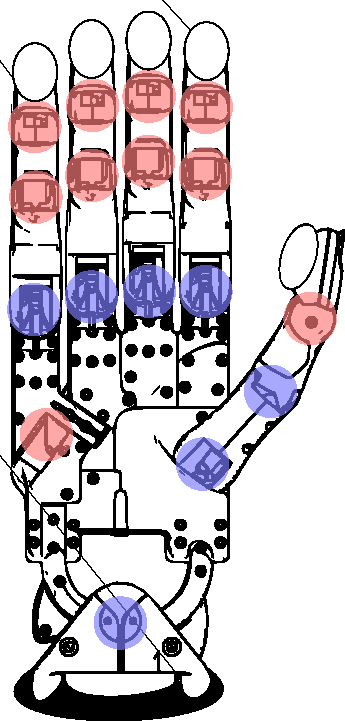
\includegraphics[height=\textwidth]{chapters/system-setup/fig/robot-hand-skeleton.pdf}
		\caption{Shadow Dexterous hand with joints color coded depending on the degrees of freedom. The total number of degrees of freedom can here be seen as \num{24}. This figure is based on~\cite{svg-robot-hand}.}
		\label{fig:robot-hand-skeleton}
	\end{subfigure}
	\hfill
	\begin{subfigure}[b]{0.48\textwidth}
		\centering
		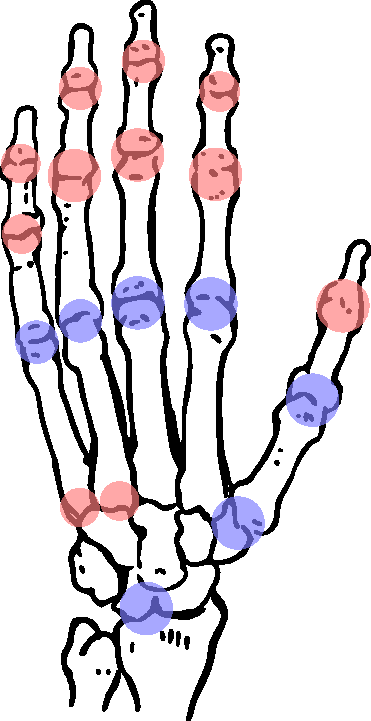
\includegraphics[height=\textwidth]{chapters/system-setup/fig/human-skeleton-hand.pdf}
		\caption{Shadow Dexterous hand with joints color coded depending on the degrees of freedom. The total number of degrees of freedom can here be seen as \num{25}~\cite{design-and-development-of-a-bilateral-therapeutic-hand-device-for-stroke-rehabilitation}. This figure is based on~\cite{svg-skeleton-hand}.}
		\label{fig:human-hand-skeleton}
	\end{subfigure}
	\caption{The Shadow Dexterous hand and a human hand red here marks a joint with \num{1} degree of freedom, while blue marks a joint with \num{2}.}
	\label{fig:hands-dof}
\end{figure}

The hand's geometry is modeled using a combination of standard shapes and custom-designed components. For example, the finger joints are modeled using a series of cylinders and spheres, which are connected by virtual tendons to simulate the motion of the real-world hand. The tactile sensors on the simulated hand, at the writing of this thesis, are purely aesthetical as representative simulated tactile sensors are yet to be supported as a standard component. To generate representative tactile data additional software is therefore required. The tactile sensors can be seen in \figref{fig:robot-hand-skeleton} as the ellipsoids mounted at each fingertip. \medskip

Multiple hand configurations are available including a left hand, right hand, and both configurations mounted on \gls{ur} manipulators~\cite{shadow-hand-configurations}. The configuration chosen for this project is a Shadow Dexterous right hand without being mounted on a manipulator. \figref{fig:simulated-robot-hand} shows the \gls{cad} model of the Shadow Dexterous Hand in simulation.

\begin{figure}[h]
	\begin{small}
		\begin{center}
			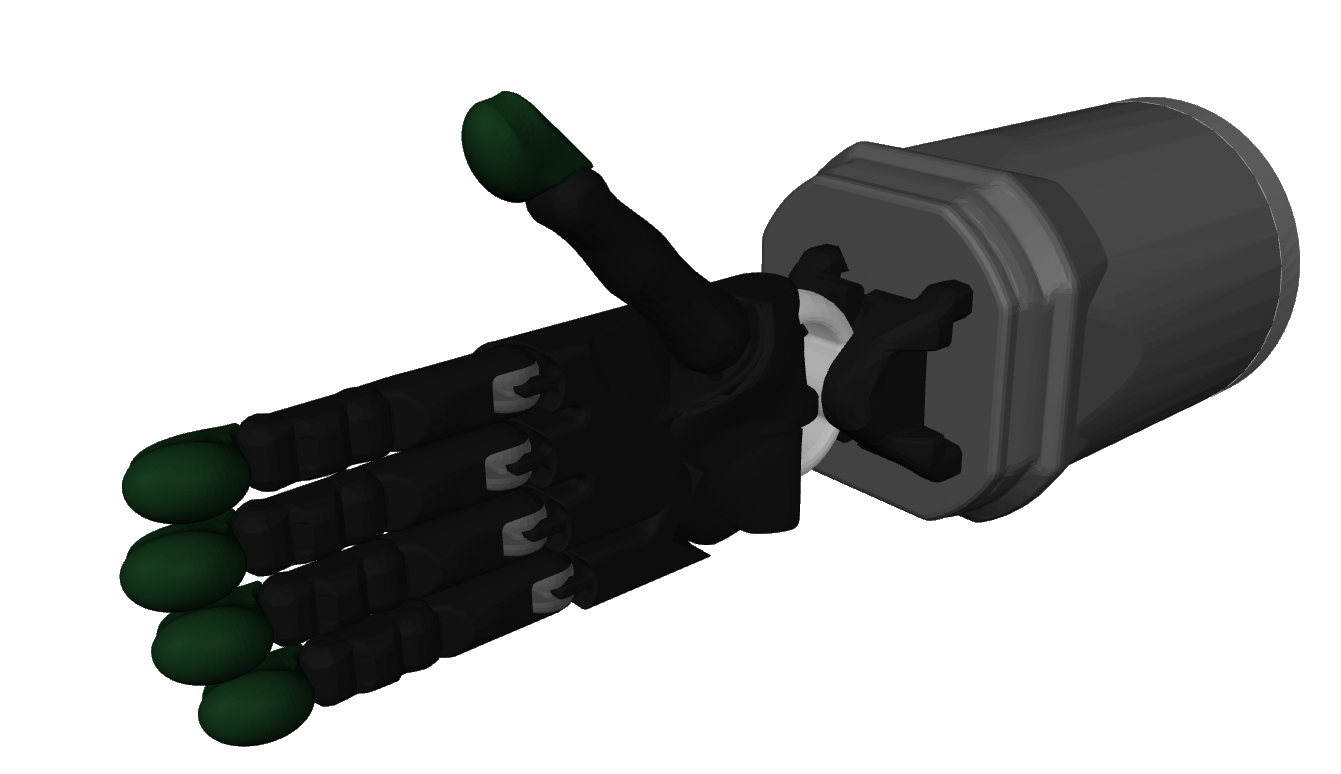
\includegraphics[width=0.6\textwidth]{chapters/system-setup/fig/simulation-robot-hand.png}
		\end{center}
		\caption{A cutout of the simulated Shadow Dexterous Hand.}
		\label{fig:simulated-robot-hand}
	\end{small}
\end{figure}

\section{Software Setup} \label{sec:system-setup-software-setup}

The software setup is shipped in a custom Ubuntu-based docker container~\cite{docker, ubuntu-docker-image} with the necessary libraries to communicate and develop applications on the simulated as well as the physical hand, wrapped within a catkin workspace~\cite{catkin}. Additionally, the container comes with common-use libraries for Python and C++ development in \gls{ros} including \texttt{numpy}\cite{numpy}, \texttt{OpenCV}~\cite{opencv} and \texttt{dynamic\_reconfiguration}~\cite{dynamic-reconfiguration}. The development environment can be seen illustrated in \figref{fig:package-diagram}. The communication between the provided \gls{ros} packages and the Gazebo simulator is achieved through the \gls{ros}-Gazebo framework. 

\begin{figure}[h]
	\begin{small}
		\begin{center}
			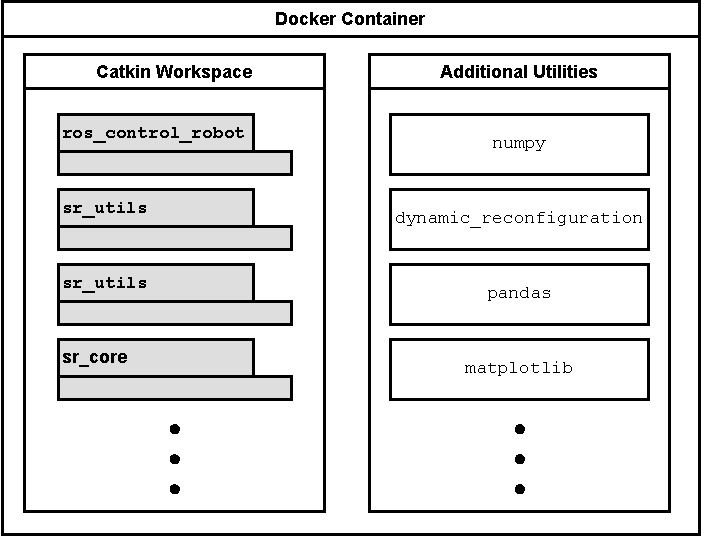
\includegraphics[width=0.6\textwidth]{chapters/system-setup/fig/init-package-diagram.pdf}
		\end{center}
		\caption{The boxes marked with grey are \gls{ros} packages, while the white are python modules.}
		\label{fig:package-diagram}
	\end{small}
\end{figure}

When communicating with the simulated Shadow Dexterous hand, the primary interface provided is the 

\texttt{SrHandCommander} which enables the definition of plans to execute and values to be read.
Plans are executed using a PID controller~\cite{controlling-the-hand}, which follows an \gls{rrt}-Connect sample-based planner by default to generate paths. Planning is done in the configuration space.

% https://shadow-robot-company-dexterous-hand.readthedocs-hosted.com/en/latest/user_guide/ed_control_description.html